\documentclass[varwidth=true, border=2pt]{standalone}

\usepackage{pgfplots}
\usepackage{tikz}

\begin{document}
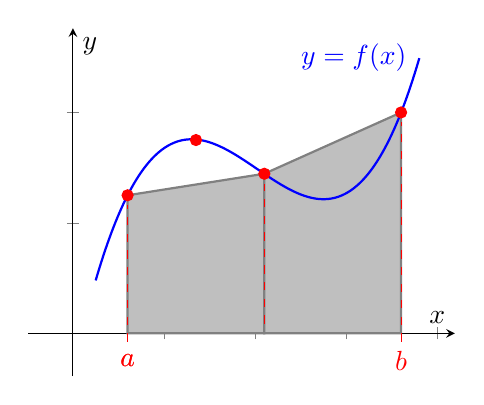
\begin{tikzpicture}
    \begin{axis}[
        legend pos=south east,
        axis x line=middle,
        axis y line=middle,
	xticklabels=\empty,
	yticklabels= \empty,
        grid = none ,
        width=7cm,
        height=6cm,
        grid style={dashed, gray!1},
        xmin=-0.5,     % start the diagram at this x-coordinate
        xmax=19,    % end   the diagram at this x-coordinate
        ymin=-0.25,     % start the diagram at this y-coordinate
        ymax= 5,   % end   the diagram at this y-coordinate
        xlabel=$x$,
        ylabel=$y$,
        enlargelimits=true,
        tension=0.08]
        
        \node(A1) at (axis cs: 3, 0){};
        \node(A2) at (axis cs: 3, 2.5){};
       \node(B1) at (axis cs: 18, 0){};        
        \node(B2) at (axis cs: 18, 4){};
         \node(MP1) at (axis cs: 10.5,0){};
         \node(MP2) at (axis cs: 10.5,2.89){};

\draw[draw = gray, thick,  fill = lightgray] (A1.center) -- (A2.center) -- (MP2.center) -- (MP1.center) -- cycle;
\draw[draw = gray, thick,  fill = lightgray] (MP1.center) -- (MP2.center) -- (B2.center) -- (B1.center) -- cycle;
  \addplot[domain=1.25:19, blue, thick,samples=250] {(x-7)*(x-10)*(x-18)/(-840)+(x-3)*(x-10)*(x-18)/88+(x-3)*(x-7)*(x-18)/(-168)+(x-3)*(x-7)*(x-10)/660 +2}; % Function
  \addplot[red, only marks, mark=*] coordinates {(3,2.5)(6.75,3.5)(10.5,2.89)(18,4)};
  \draw [red,dashed] (axis cs: 3,-0.15) -- (A2);
  \draw [red,dashed] (MP1) -- (MP2);
  \draw [red,dashed] (axis cs: 18,-0.15) -- (B2);
  

	\node(a)[red] at (axis cs: 3,-0.5){$a$};
	\node(b)[red] at (axis cs: 18,-0.5){$b$};
	\node(a)[red] at (axis cs: 3,-0.5){$a$};
	\node(yf)[blue] at (axis cs: 15.4,5){$y=f(x)$};
    \end{axis}
\end{tikzpicture}
\end{document}